\section{Validation of the $A$-coefficients consistent with \texttt{PDF4LHC21\_40} and at $\sqrt{s}=13$ and $14$ TeV}
\label{sec:validation_transport}
%The transport $K$-factors needed for the coefficients at $13$ and $14$ TeV are obtained with the generation at both COM energies of all basis points in the full 9D-basis shown in Table~\ref{tab:smeft_basis_9d}. The factors are then obtained by using the coefficients obtained through the fit made at $13.6$ TeV to predict the distributions in all bins for all basis points, and then extracting the differences that correct for the MC distributions at $13$ and $14$ TeV. 

\begin{figure}[h!]
    \centering    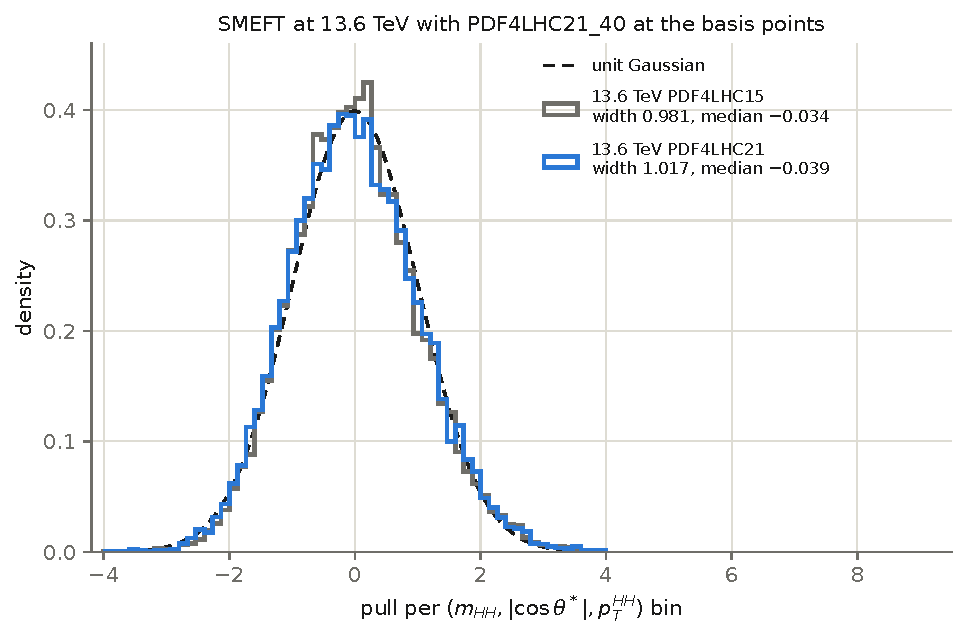
\includegraphics[width=0.8\linewidth]{plots/SMEFT_pulls_13p6TeV_PDF4LHC15_vs_PDF4LHC21.pdf}
    \caption{Pull of the PDF-transported $A$-coefficients per $(\mHH, |\cos\theta^*|, \pt^{HH})$ bin, on the basis points, against a unit Gaussian (dashed). The gray distribution correspond to the coefficients consistent with \texttt{PDF4LHC15} and applied to the basis generated at the same PDF set. Similarly, the blue distribution correspond to the coefficients consistent with \texttt{PDF4LHC21} and applied to the basis points generated at the same PDF set.}
    \label{fig:PDFchange}
\end{figure}
\begin{figure}[h!]
    \centering    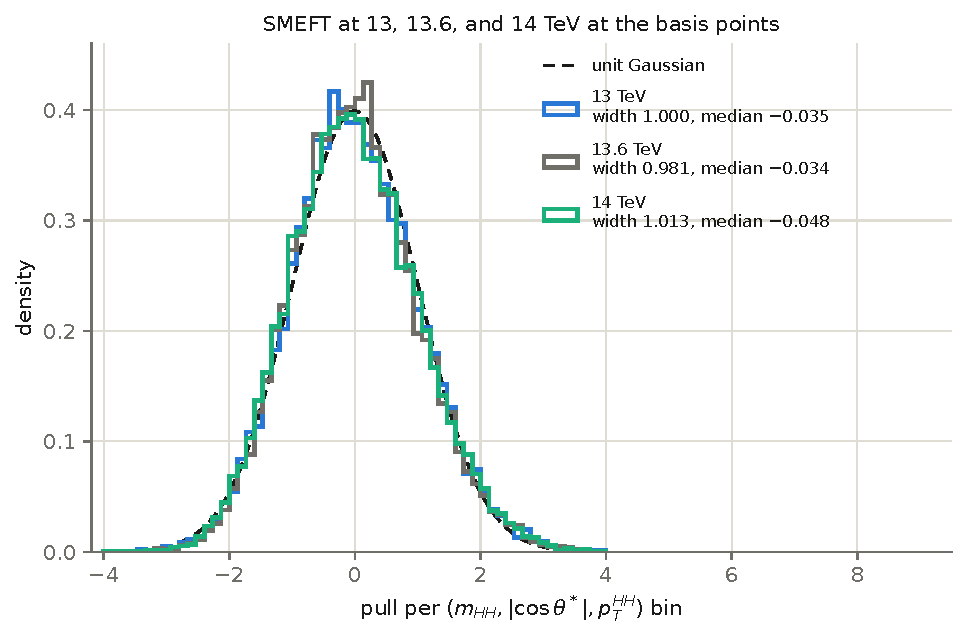
\includegraphics[width=0.8\linewidth]{plots/SMEFT_pulls_13_13p6_14TeV.pdf}
    \caption{Pull of the transported $A$-coefficients per $(\mHH, |\cos\theta^*|, \pt^{HH})$ bin, on the basis points, against a unit Gaussian (dashed).}
    \label{fig:COMEchange}
\end{figure}

In order to validate the transported coefficients, additional samples are generated at the basis points (see Table \ref{tab:smeft_basis_9d}) with the PDF set \texttt{PDF4LHC21\_40} and at $\sqrt{s}=13$ and $14$ TeV. The effects of the PDF change is observed in Figure \ref{fig:PDFchange}, where gaussian-like properties are observed in both the pull distributions, indicating consistent modeling for each of the PDF sets. Finally, the results with all COM energies are exhibited in Figure~\ref{fig:COMEchange}. By comparing the $13.6$ TeV results (fitted coefficients) with the other COM energies (transported coefficients), the same level of agreement is observed. %Figure \ref{fig:pth2} shows some distributions using ELR at both COM energies.

%\begin{figure}[h!]
%    \centering    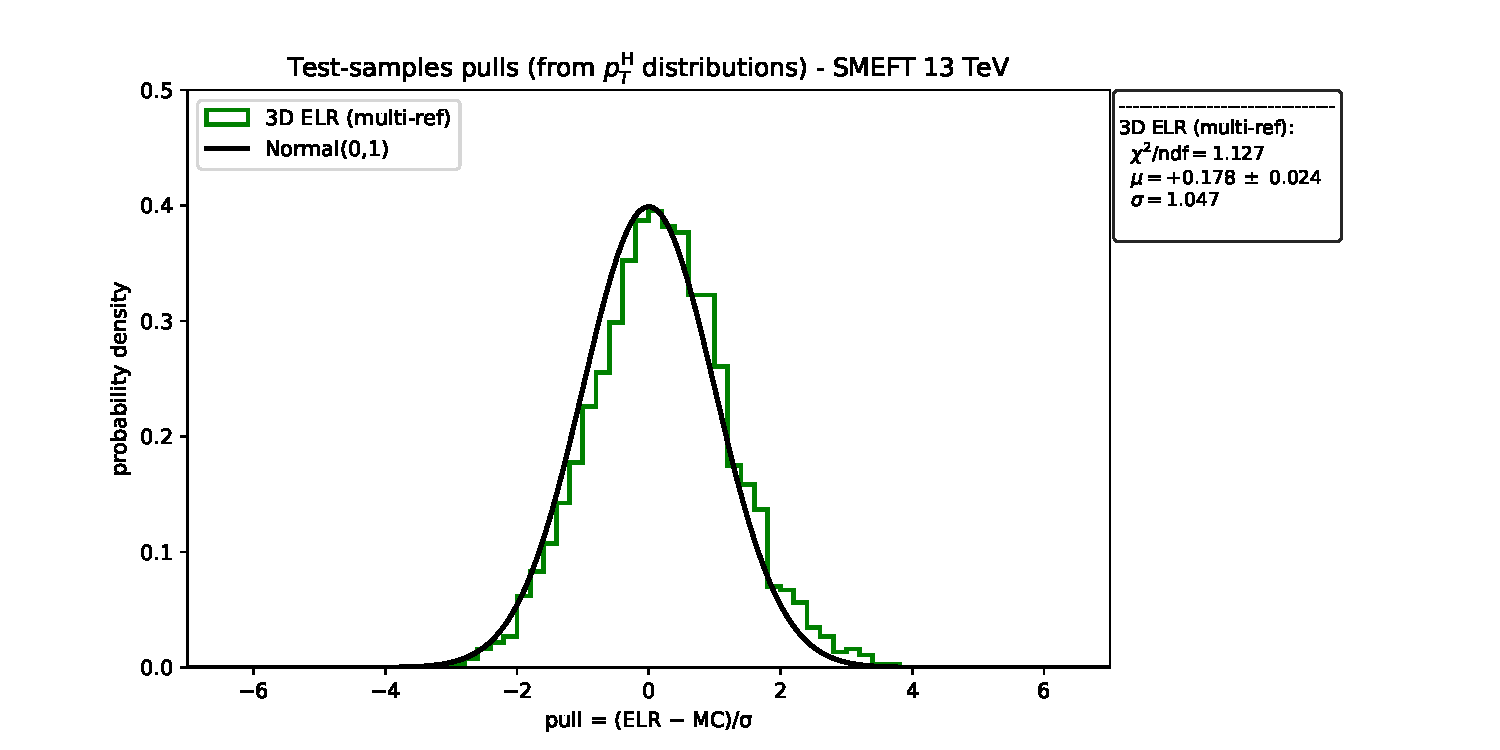
\includegraphics[width=1\linewidth]{plots/pulls_pth_3d_SMEFT13TeV_transport_pt500_plot_2.pdf}
%    \caption{Pulls obtained with all test-samples in all $p^\text{H}_T$ bins in SMEFT. The statistical parameters $\{\chi^2,\mu,\sigma\}$ are very similar to those at obtained at $13.6$ TeV (see Fig.~\ref{fig:stats}), therefore validating the transport among coefficients in different COM energies.}
%    \label{fig:stats2}
%\end{figure}

%\begin{figure}[h!]
%  \begin{minipage}[b]{0.495\linewidth}
%    \centering
%    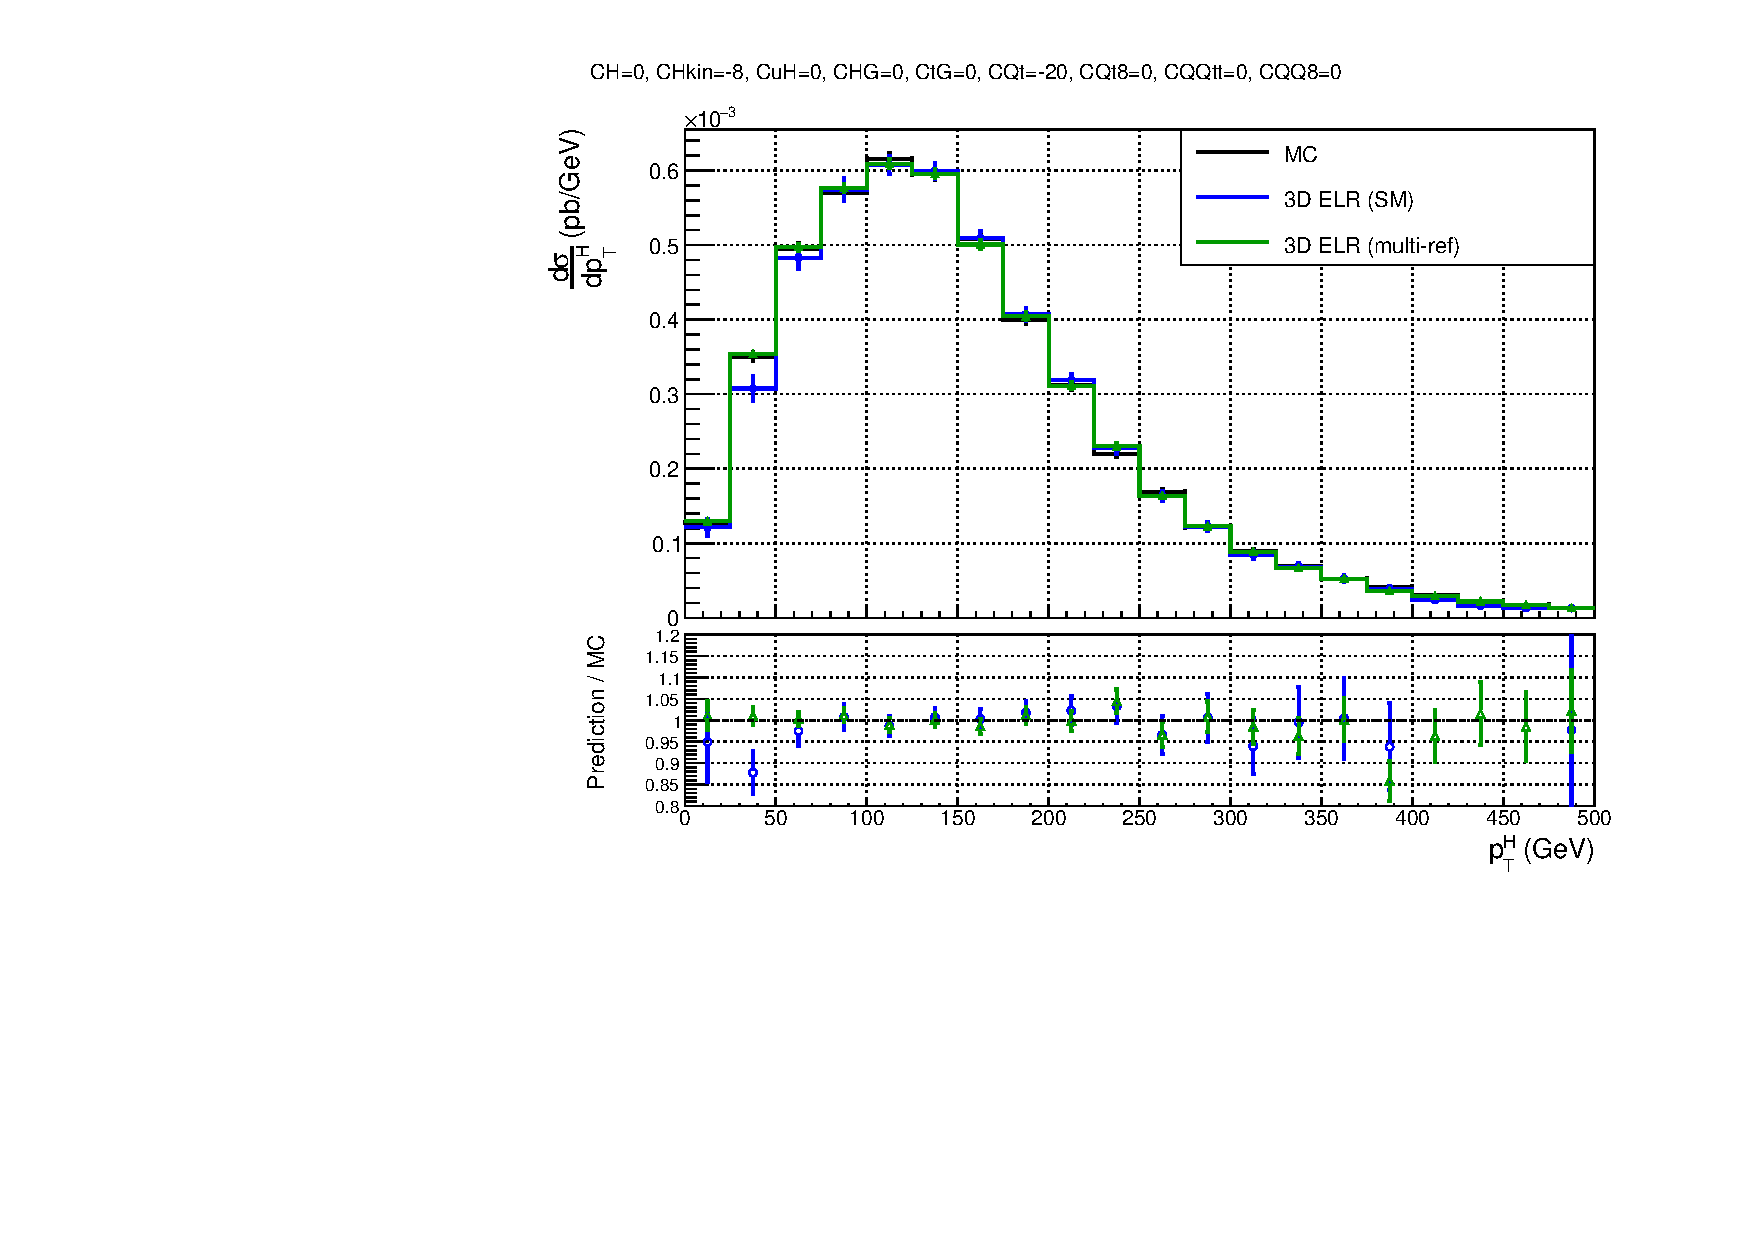
\includegraphics[width=\linewidth]{plots/pth_3d_9D_13TeV_transport_27_CH_0.0_CHbox_-8.0_CuH_0.0_CHG_0.0_CtG_0.0_CQt_-20.0_CQt8_0.0_CQQtt_0.0_CQQ8_0.0.pdf}
%  \end{minipage}
%  \hfill
%  \begin{minipage}[b]{0.495\linewidth}
%    \centering
%    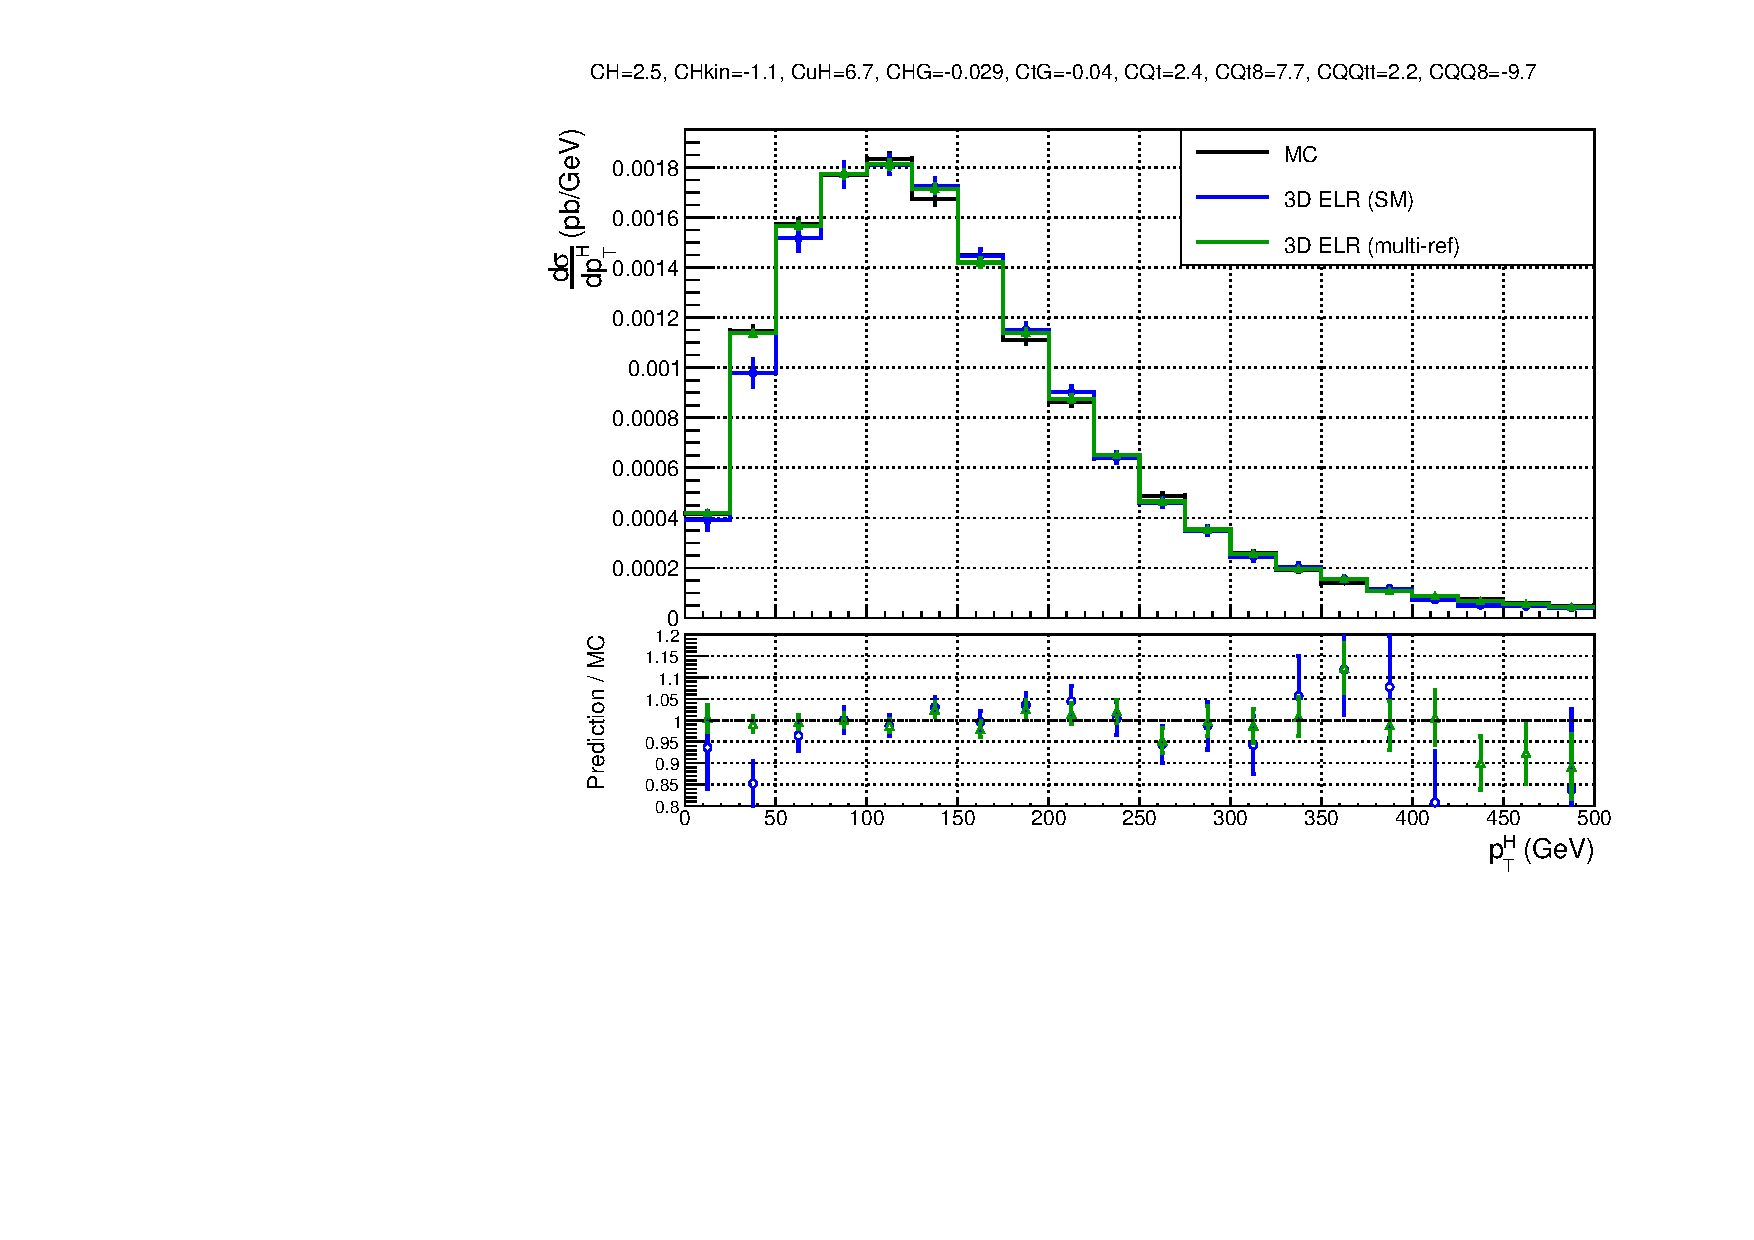
\includegraphics[width=\linewidth]{plots/pth_13TeV_transport_72_CH_2.48_CHbox_-1.12_CuH_6.66_CHG_-0.029_CtG_-0.040_CQt_2.3_CQt8_7.66_CQQtt_2.16_CQQ8_-9.69282.pdf}
%  \end{minipage}
%  \caption{Higgs transverse momenta distributions for some of the test-samples generated at $\sqrt{s}=13$ TeV. The closure is very similar to the case at $13.6$ TeV.}
%  \label{fig:pth2}
%\end{figure}
%\begin{figure}[h!]
%  \centering
  % First group: 2 x 2
%  \begin{minipage}[b]{0.495\linewidth}
%    \centering
    %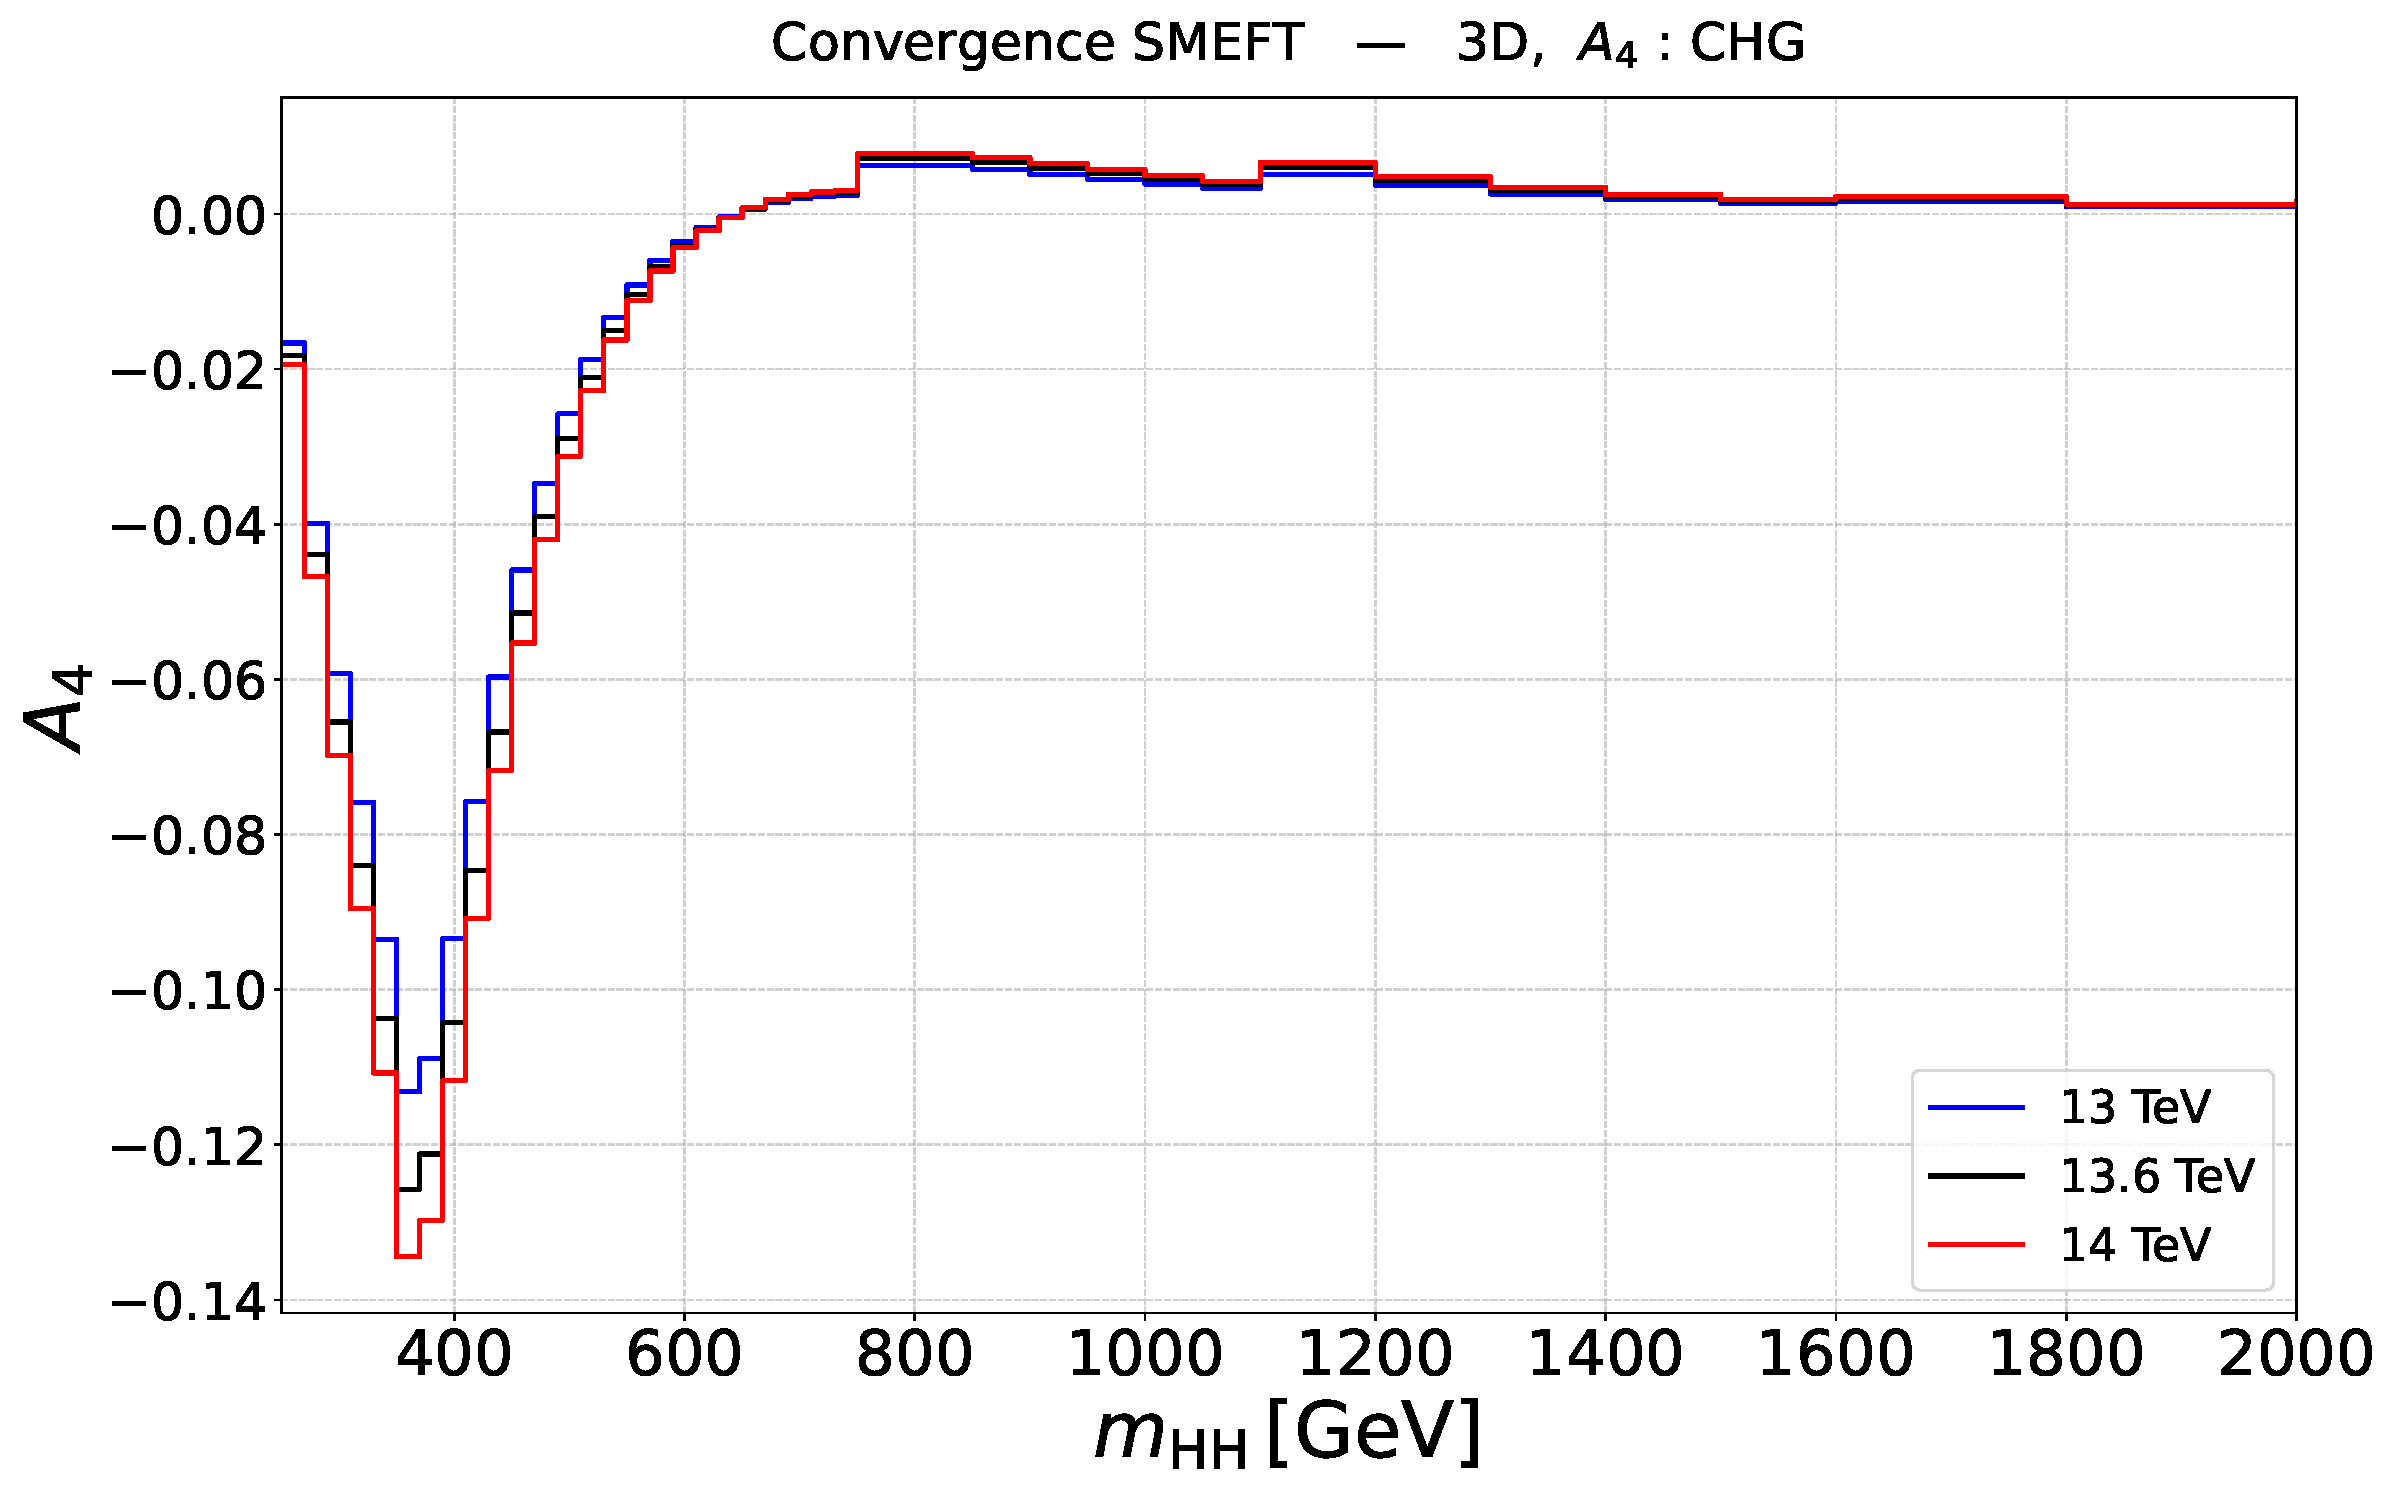
\includegraphics[width=\linewidth]{plots/plot_param4_250_2000_3d_energy_13_13p6_14TeV.pdf}
  %\end{minipage}
  %\hfill
  %\begin{minipage}[b]{0.495\linewidth}
   % \centering
    %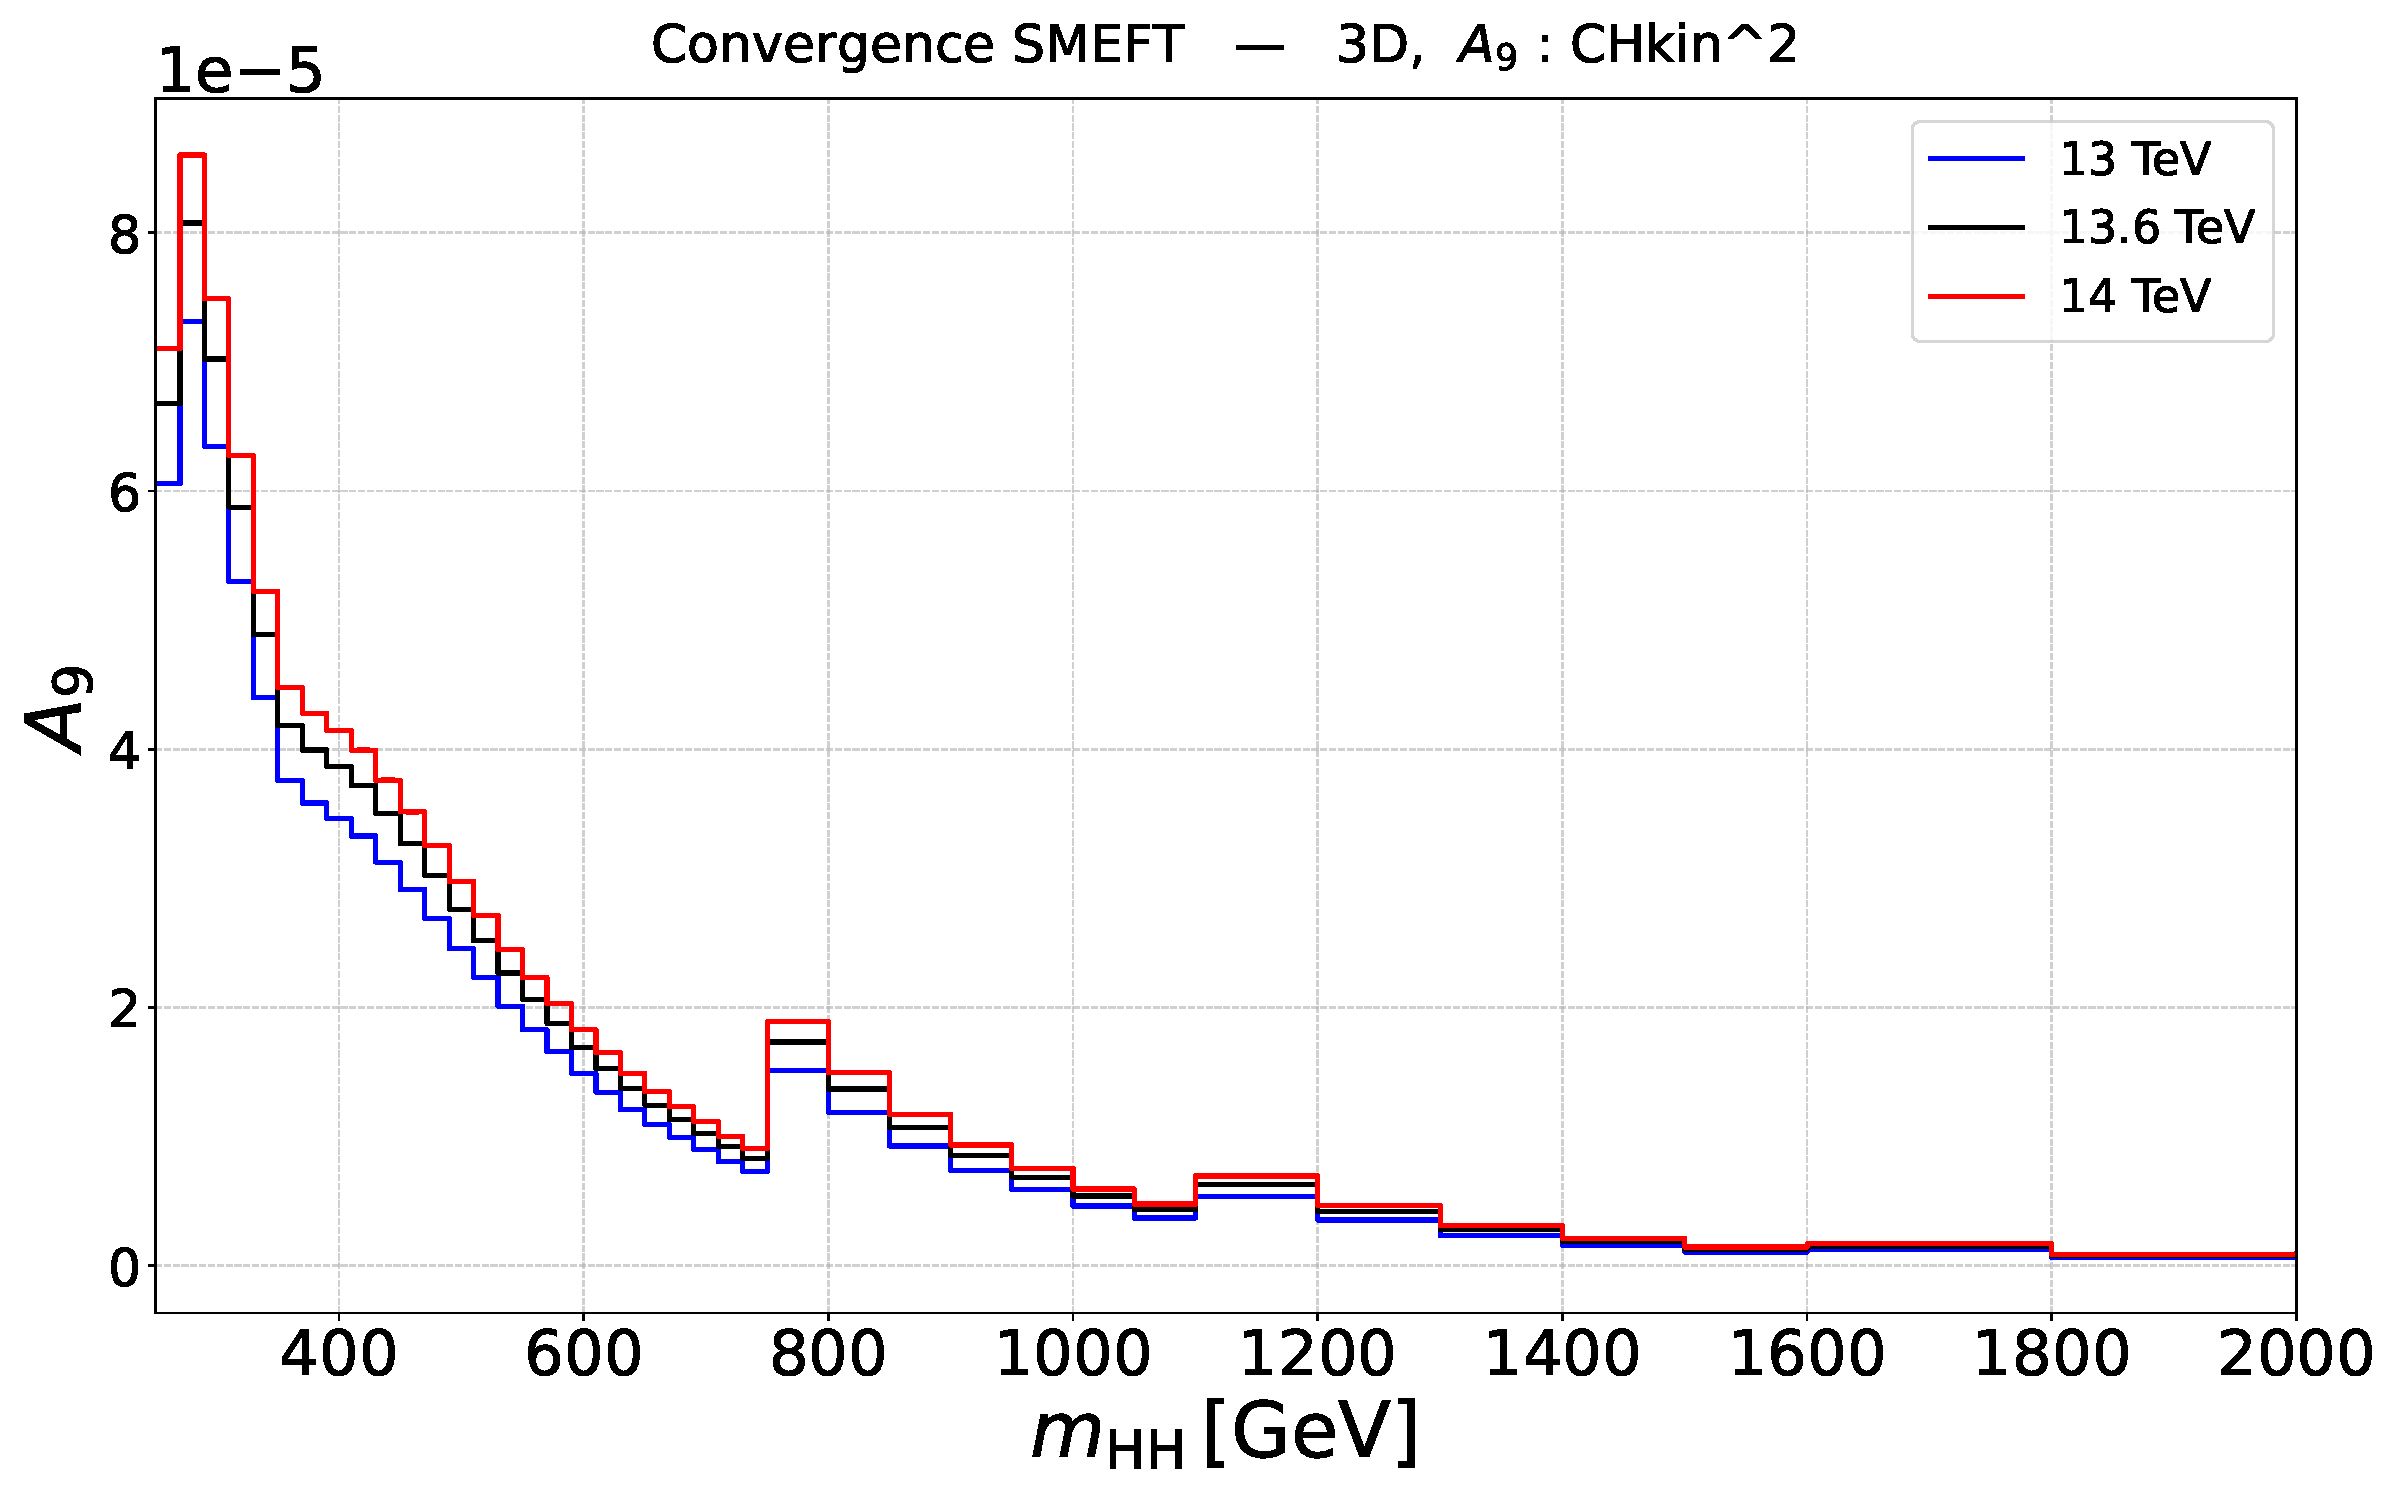
\includegraphics[width=\linew%idth]{plots/plot_param9_250_2000_3d_energy_13_13p6_14TeV.pdf}
  %\end{minipage}
  %\vspace{0.5em}
  %\begin{minipage}[b]{0.495\linewidth}
   % \centering
    %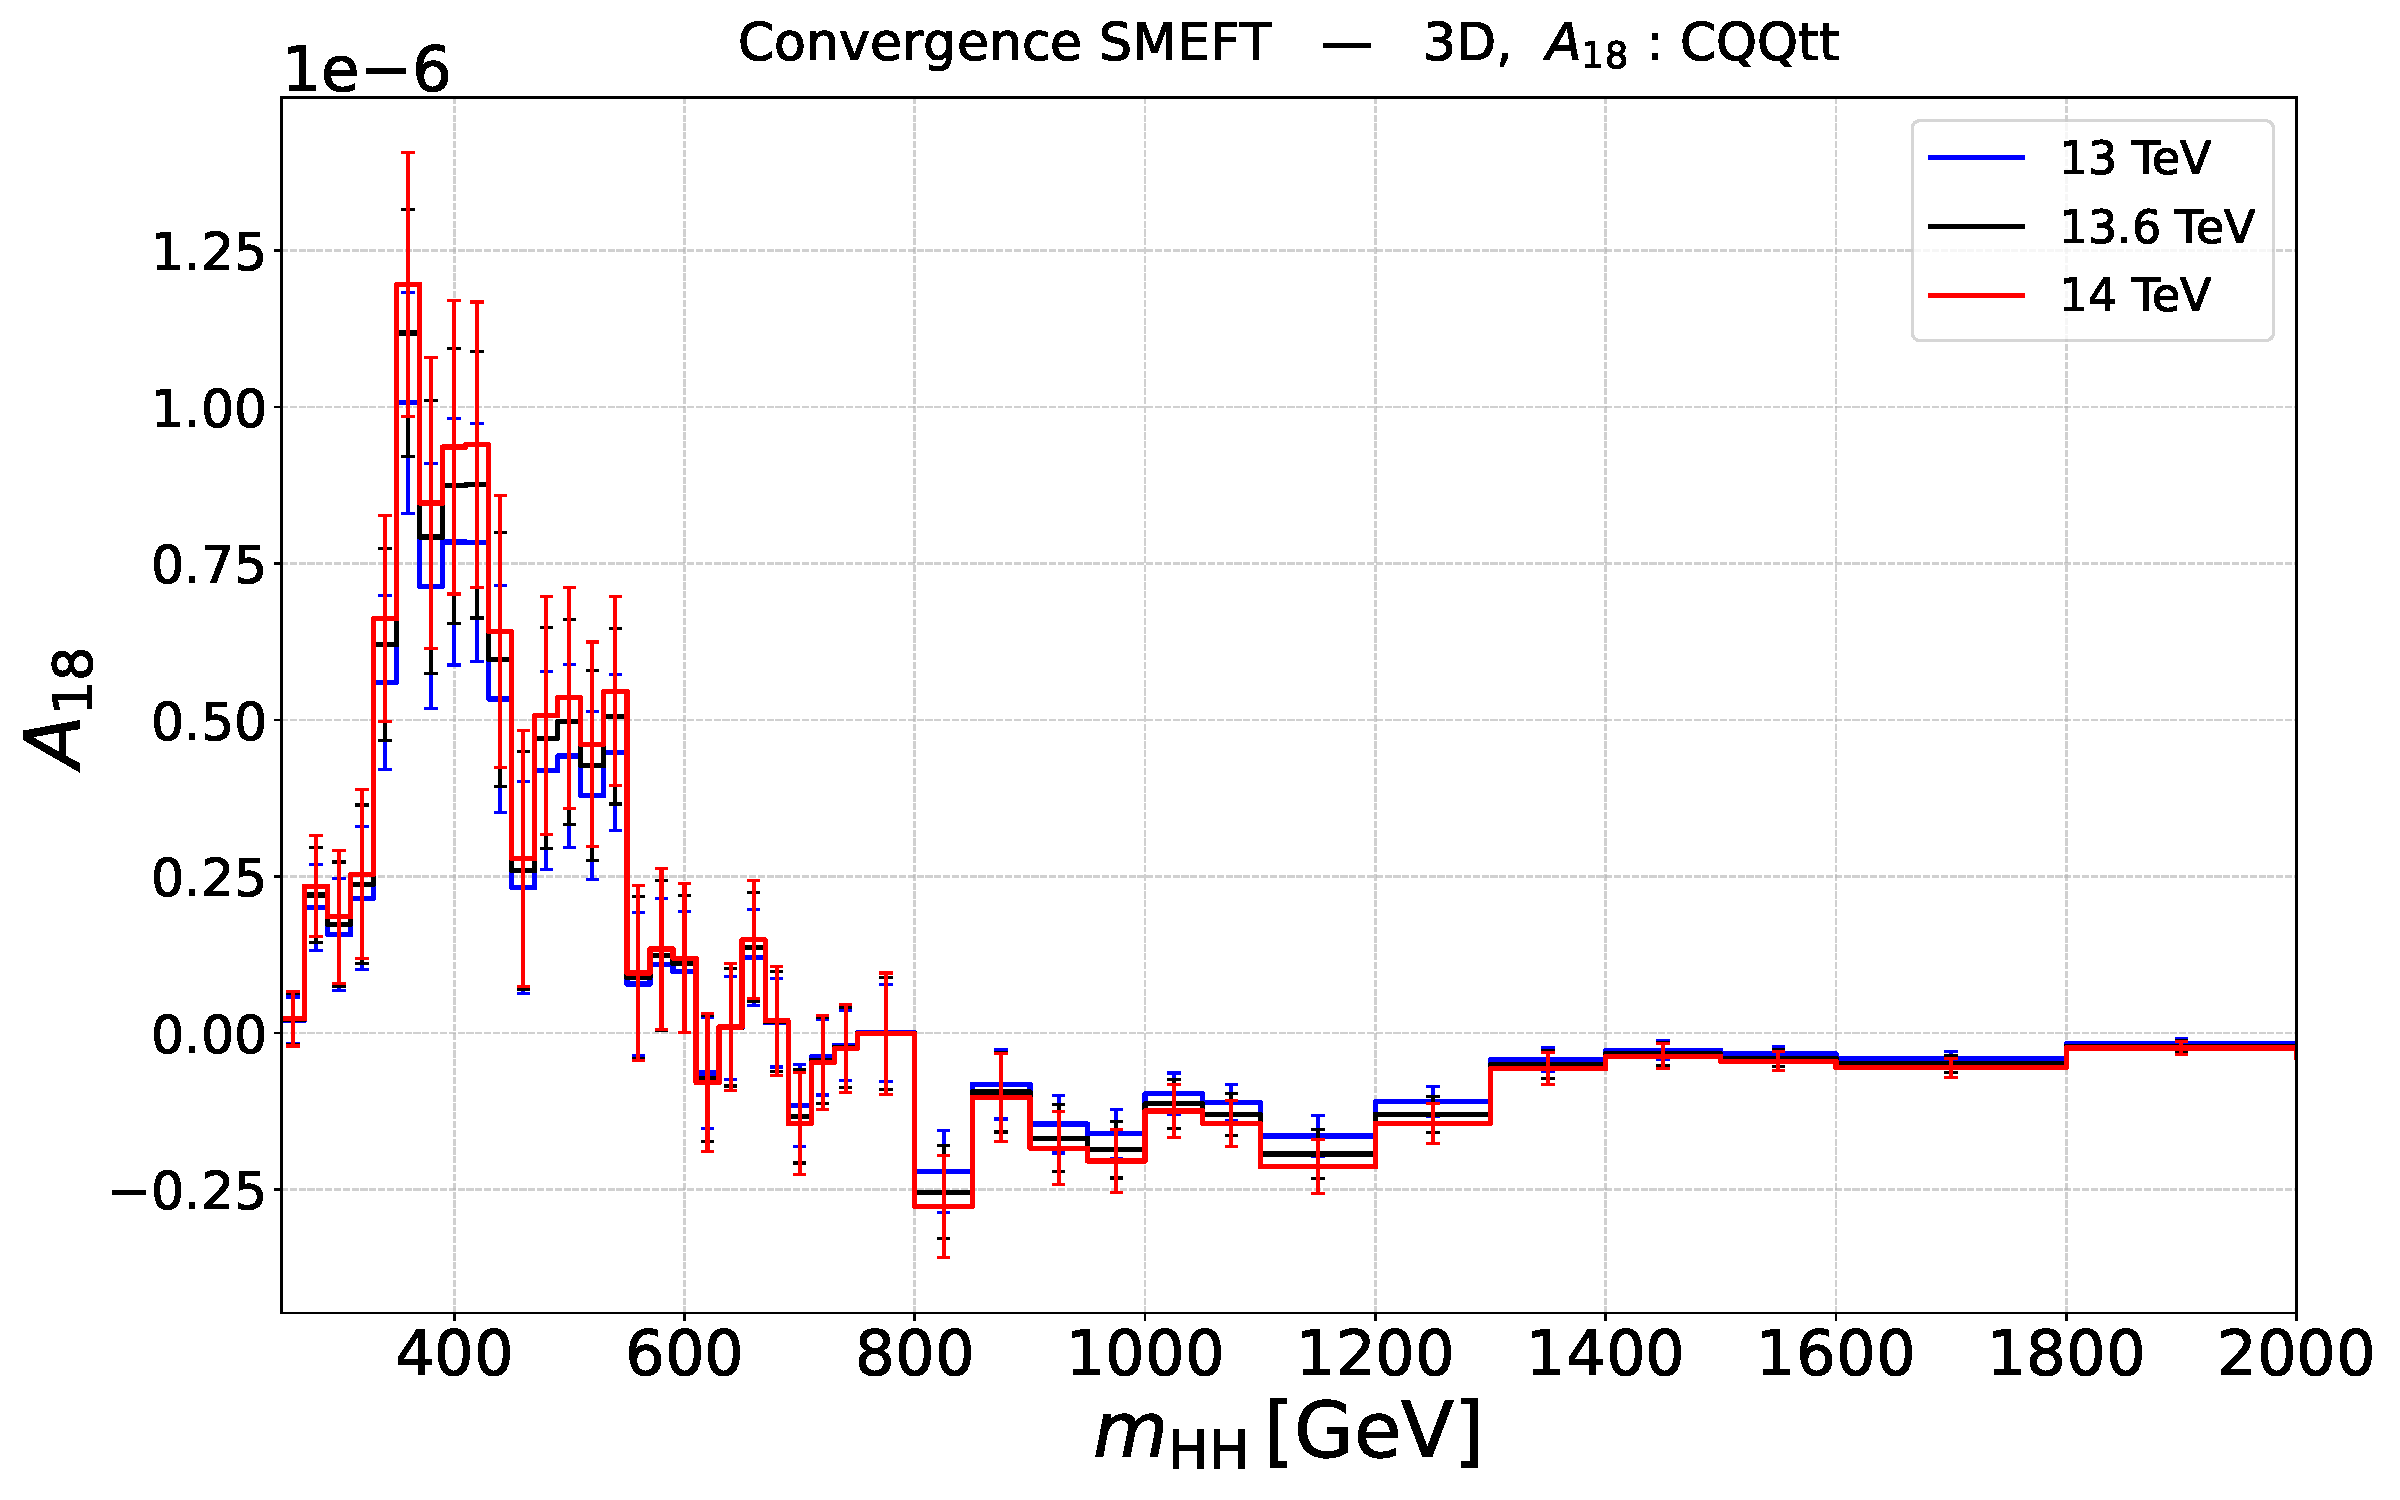
\includegraphics[width=\linew%idth]{plots/plot_param18_250_2000_3d_energy_13_13p6_14TeV.pdf}
  %\end{minipage}
  %\hfill
  %\begin{minipage}[b]{0.495\linewidth}
  %  \centering
    %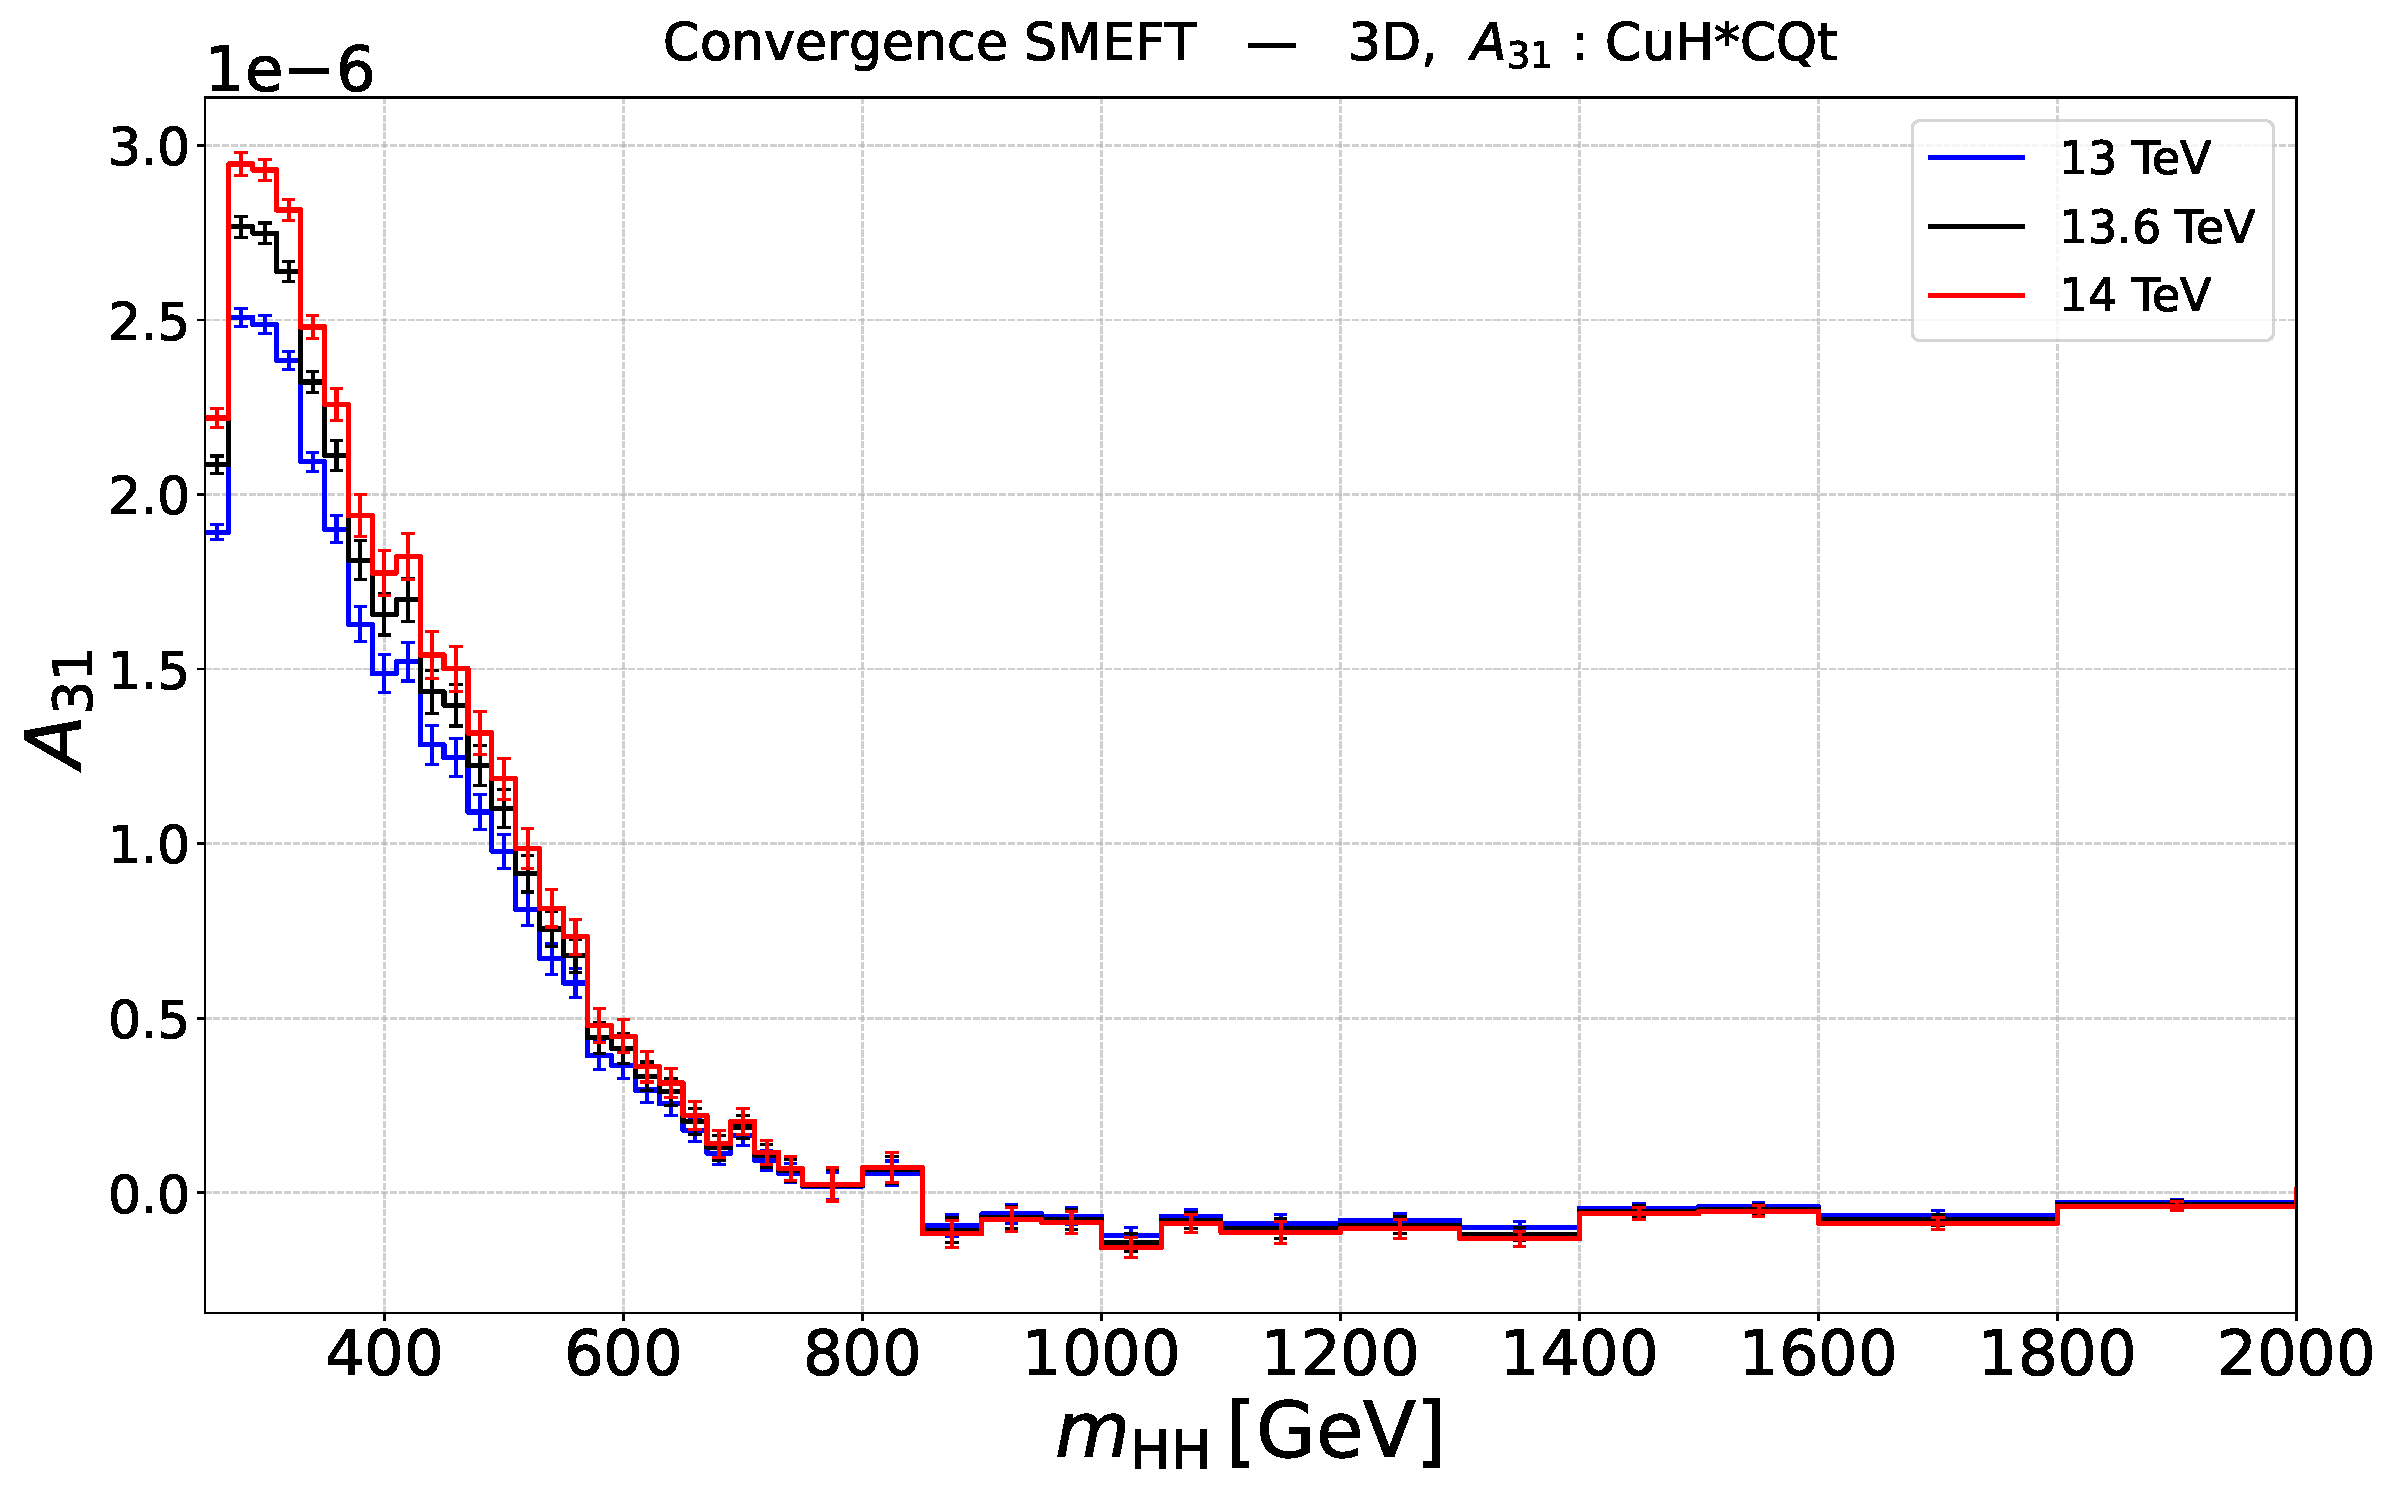
\includegraphics[width=\linewidth]{plots/plot_param31_250_2000_3d_energy_13_13p6_14TeV.pdf}
  %\end{minipage}
  %\caption{Convergence of the 3D $A$-coefficients projected into $m_{\text{HH}}$, for the three COM energies. The upper panel shows coefficients arising from leading-operator terms, while the lower panel shows coefficients arising from subleading and leading$\times$subleading terms.}
  %\label{fig:convergence_allCOM}
%\end{figure}